\documentclass[11pt, conference, compsoc, twoside]{IEEEtran}
% JIKI template packages (AuthorGuideline_JIKI.zip / mainTemplate_JIKI.tex)
\usepackage[numbers,sort&compress]{natbib}
\usepackage[labelsep=period,labelfont=bf,justification=justified,font=small]{caption}
\usepackage{balance}
\usepackage{graphicx}
\usepackage{amsmath}
\usepackage{amssymb}
\usepackage{array}
\usepackage{booktabs}
\usepackage{tikz}
\usetikzlibrary{shadows, arrows.meta, positioning, fit, backgrounds, shapes.geometric, arrows}
\usepackage[english]{babel}
\usepackage{url}
\usepackage{listings}
\usepackage{inconsolata}
\lstset{basicstyle=\ttfamily}
\usepackage[bottom]{footmisc}
\setlength{\footnotemargin}{0.3em}
\hyphenation{op-tical networks semi-conduc-tor}
\hyphenation{PASCAL}
\usepackage[a4paper, top=3cm,bottom=3cm,left=3cm,right=3cm]{geometry}
\usepackage{fancyhdr}
\setlength{\headheight}{22pt}
\pagestyle{fancy}
\fancyhf{}
\setcounter{page}{1}
\fancypagestyle{firststyle}
{
   \fancyhf{}
   \chead{Jurnal Ilmu Komputer dan Informasi (Journal of Computer Science and Information) \\ 15/1 (2022), xx-xx. DOI: \url{http://dx.doi.org/10.21609/jiki.v15i1.xxx}}
   \fancyfoot[C]{\thepage}
}
\renewcommand{\headrulewidth}{0pt}
\fancyhead[LE]{\thepage \textbf{\space \textit{Jurnal Ilmu Komputer dan Informasi (Journal of Computer Science and Information),}} \textit{volume 15,} \\ \textit{ \textrm{ } issue 1, February 2022}}
\fancyhead[LO]{\textit{Anonymous et.al., Delta BPTT Add-Only Backpropagation}}
\fancyhead[RO]{\thepage}
\usepackage{hyperref}
\renewcommand{\UrlBreaks}{\do\-}
\makeatletter
\def\footnoterule{\kern-3\p@
  \hrule \@width 2in \kern 2.6\p@}
\makeatother
\def\figurename{Figure}%
\def\tablename{Table}%
% Math notation commands (adapted from dlbook_notation style)
% Local copy so the revised paper is self-contained and compilable.
\newcommand{\bm}{\boldsymbol}

% Matrices / vectors used in the paper
\newcommand{\mX}{\boldsymbol{X}}
\newcommand{\mW}{\boldsymbol{W}}
\newcommand{\mV}{\boldsymbol{V}}
\newcommand{\mS}{\boldsymbol{S}}
\newcommand{\mE}{\boldsymbol{E}}
\newcommand{\mQ}{\boldsymbol{Q}}
\newcommand{\mK}{\boldsymbol{K}}
\newcommand{\mM}{\boldsymbol{M}}
\newcommand{\mD}{\boldsymbol{D}}
\newcommand{\mU}{\boldsymbol{U}}
\newcommand{\mT}{\boldsymbol{T}}
\newcommand{\mP}{\boldsymbol{P}}

\widowpenalty=10000
\clubpenalty=10000

\begin{document}

\title{Delta BPTT: Efficient Add-Only Backpropagation Through Time for Spiking Sequence Representations}

\author{\IEEEauthorblockN{Anonymous Authors}\\
\IEEEauthorblockA{\normalfont Anonymous Affiliations\\
anonymous@anonymous.com\\
}}

\twocolumn[
{\csname @twocolumnfalse\endcsname \maketitle}
{\csname @twocolumnfalse\endcsname
	\renewcommand{\abstractname}{Abstract}
	\begin{abstract}
		\noindent
		\normalfont
		Spiking Neural Networks (SNNs) offer an energy-efficient alternative to deep neural networks through discrete, event-driven spikes. However, training SNNs on temporal tasks with Backpropagation Through Time (BPTT) re-introduces dense floating-point Multiply-Accumulate (MAC) operations in the backward pass, negating these efficiency gains. We introduce \textbf{Delta BPTT}, an Add-Only gradient routing rule that exploits the strict binary nature of forward spike events to gate weight-gradient accumulation as sparse, conditional additions, eliminating dense MACs in both the recurrent forward projection and parameter-gradient phases. A $65$K-parameter recurrent embedder trained with Delta BPTT reaches $0.5046$ Pearson on the ALL-STS human benchmark aggregate ($0.8031$ teacher distillation correlation) and $0.7651$ Pearson on STS-B --- $93.4\%$ of SpikingBERT's reported STS-B correlation while using roughly $770\times$ fewer parameters and requiring no GPU. Replacing explicit spatial attention with recurrent temporal pooling trained via Delta BPTT delivers a $4.13\times$ reduction in training time and a $2.09\times$ reduction in inference latency, demonstrating that structurally optimized Add-Only temporal gradients offer a highly efficient alternative to spatial routing in neuromorphic sequence representation.
		\\\\
		\noindent
		\textbf{Keywords}: Spiking Neural Networks, Sequence Representation, Backpropagation Through Time, Energy Efficiency. \\\\
	\end{abstract}
}
]

\IEEEpeerreviewmaketitle
\thispagestyle{firststyle}

\section{Introduction}

Neuromorphic computing aims to deliver brain-inspired, low-power intelligence by processing information as sparse, event-driven spikes rather than dense matrix algebra \cite{roy2019towards}. In the domain of natural language processing, dense sentence embedders such as SBERT \cite{reimers2019sentence} are dominated by the matrix multiplications of standard Scaled Dot-Product Attention \cite{vaswani2017attention}. Although numerous efficient Transformer variants reduce this quadratic $\mathcal{O}(L^2)$ complexity \cite{tay2022efficient}, they still rely fundamentally on continuous floating-point operations. Spiking Neural Networks (SNNs) alleviate this constraint by operating on sparse, event-driven additions rather than multiplications, making them well suited to highly parallel neuromorphic hardware. Recent neuromorphic NLP work has therefore focused on porting self-attention to the spiking domain, most notably SpikFormer \cite{zhou2023spikformer} and SpikeGPT \cite{zhu2023spikegpt}, and frameworks such as SpikingJelly \cite{fang2023spikingjelly} have accelerated the validation of surrogate-gradient methods in deep architectures.

However, a critical and often overlooked bottleneck persists not in the \textit{forward} pass --- where spike-driven sparsity is well established --- but in the \textit{backward} pass. Standard BPTT with surrogate gradients \cite{neftci2019surrogate} requires continuous, floating-point gradient matrices to flow backward through the discrete network, re-introducing dense MAC operations during weight-gradient computation and effectively negating the training-time efficiency gains that motivate spiking architectures. Forcibly mapping continuous $\mathcal{O}(L^2)$ spatial attention into the discrete spiking domain further inflates this overhead. This raises two fundamental questions: \textit{(1)~Can weight-gradient accumulation in SNN training be made as sparse as the forward pass? (2)~Are explicit spatial attention mechanisms truly necessary for sequence representation, or can the native temporal recurrence of SNNs, when paired with an efficient learning rule, suffice?}

In this study we answer both questions affirmatively by proposing \textbf{Delta BPTT}, an Add-Only recurrent gradient routing mechanism. By exploiting the binary spike indicator $\mathbb{I}[S^{(t)} = 1]$ as a natural gate on gradient flow, the dense backward MAC operation $\mX^T \cdot \bm{\delta}$ is entirely replaced by sparse conditional accumulations, shifting the computational profile of weight updates from dense matrix algebra to event-driven additions. Our results demonstrate that the native temporal integration of a recurrent pooler trained with Delta BPTT is sufficient for encoding sentence-level semantics, achieving $93.4\%$ of SpikingBERT's reported STS-B correlation \cite{bal2024spikingbert} while using $770\times$ fewer parameters and requiring no GPU.

\subsection{Contributions}
Our primary contribution is the proposal and rigorous evaluation of \textbf{Delta BPTT}, an Add-Only gradient routing technique for SNNs. By gating parameter updates exclusively through binary spike indicators, Delta BPTT eliminates floating-point matrix multiplications during weight-gradient computation, achieving matching forward and backward sparsity. This minimalist architecture achieves comparable semantic fidelity to spatial-attention baselines while offering a $4.13\times$ reduction in training time and a $2.09\times$ reduction in inference latency. To support and evaluate this primary algorithm, we contribute:
\begin{itemize}
    \item a mathematical formulation of Spike-Driven Spike-Overlap Attention, which serves as a comparative baseline exposing the computational bottlenecks of spatial routing in SNNs;
    \item \textbf{Hyperpolarized Padding}, an SNN-native sequence padding mechanism that forces padding tokens into a negative refractory state to prevent noise accumulation;
    \item a \textbf{formal complexity derivation and step-by-step energy estimation} proving the $\mathcal{O}(L)$ scaling advantage over $\mathcal{O}(L^2)$ attention;
    \item an \textbf{empirical comparison against a dense LSTM baseline}, demonstrating higher semantic fidelity at $2.13\times$ lower training time;
    \item a \textbf{comprehensive multi-protocol evaluation}, including architectural ablation, distillation fidelity, zero-shot task performance, a training-objective comparison, and dataset specifications for reproducibility.
\end{itemize}

The remainder of this paper is organized as follows. Section 2 reviews the background on spiking language models, efficient sentence embedding, and energy accounting for SNNs. Section 3 presents the Delta BPTT methodology and its formal computational complexity analysis. Section 4 details the experimental evaluation, including dimensionality scaling, architectural ablations, and zero-shot generalization. Section 5 discusses the implications of our findings, Section 6 states the limitations, and Section 7 concludes.

\section{Background}

\subsection{Spiking Neural Networks for Language}
A line of recent work has ported Transformer primitives into the spiking domain. SpikFormer \cite{zhou2023spikformer} introduced spike-driven self-attention for vision, and SpikeGPT \cite{zhu2023spikegpt} scaled spiking architectures to generative language modeling with up to $216$M parameters. For encoder-style representations, SpikeBERT \cite{lv2023spikebert} applies two-stage knowledge distillation from BERT, while SpikingBERT \cite{bal2024spikingbert} integrates spiking neurons with BERT-style pretraining and reports GLUE results --- including a Spearman correlation of $0.819$ on STS-B --- with approximately $50$M parameters; Spikingformer \cite{zhou2025spikingformer} stabilizes spike-driven residual learning and reports $0.545$ on STS-B with $66$M parameters. Two observations motivate our study. First, all of these models retain an explicit $\mathcal{O}(L^2)$ attention mechanism that dominates their operation counts. Second, none of them target \textit{sentence embeddings} or evaluate on the standard STS suite (STS-12 through STS-16, STS-B, SICK-R) against human judgments; to our knowledge, our $65$K-parameter recurrent embedder is the first SNN evaluated directly on this suite.

\subsection{Efficient Sentence Embedding}
Dense sentence embedders are typically obtained by fine-tuning pretrained encoders with siamese \cite{reimers2019sentence} or contrastive \cite{gao2021simcse} objectives and compressed via knowledge distillation \cite{hinton2015distilling, sanh2019distilbert, wang2020minilm}. These models define the accuracy frontier --- DistilBERT reports $0.869$ Spearman on STS-B \cite{sanh2019distilbert} --- but rely fundamentally on continuous floating-point matrix multiplications. Static embeddings with mean pooling (Word2Vec, GloVe) remain competitive low-cost baselines and are included in our evaluation. The standard evaluation convention for this task family is Spearman rank correlation against human gold labels \cite{muennighoff2022mteb, cer2017semeval}, which we adopt for the task-performance track.

\subsection{Energy Accounting for SNNs}
SNN efficiency claims conventionally rely on operation counting: spike-driven accumulate operations (SOPs/ACs) are contrasted with multiply--accumulate operations (MACs), weighted by the $45$\,nm energy figures of \cite{horowitz2014computing} ($0.9$\,pJ per 32-bit accumulation versus $4.6$\,pJ per 32-bit MAC) \cite{zhou2023spikformer, fang2023spikingjelly}. This proxy omits memory access and data movement, which can dominate real energy budgets. Crucially, existing analyses focus exclusively on the \textit{forward} pass; the backward pass of BPTT is tacitly assumed to require dense MACs. Delta BPTT addresses this gap directly by extending spike-driven sparsity into gradient computation. We therefore report both the theoretical proxy and measured CPU latency, treating the proxy strictly as an upper bound.

\section{Methodology: Delta BPTT and Architectural Dynamics}

\begin{figure*}[!t]
\begin{center}
\resizebox{0.9\textwidth}{!}{%
\begin{tikzpicture}[
    font=\sffamily,
    base/.style={rectangle, rounded corners, draw=black!60, thick, minimum height=3em, align=center, fill=white, drop shadow={opacity=0.1, shadow xshift=0.05cm, shadow yshift=-0.05cm}},
    input/.style={base, fill=blue!5, text width=18em},
    spike/.style={base, fill=orange!5, text width=16em},
    pooler/.style={base, fill=teal!5, text width=14em, minimum height=4em, draw=teal!80!black},
    attn/.style={base, fill=red!5, text width=14em, minimum height=4em, draw=red!80!black},
    output/.style={base, fill=purple!5, text width=16em},
    arrow/.style={-{Stealth[length=2mm]}, thick, draw=black!70},
    dashed_arrow/.style={-{Stealth[length=2mm]}, dashed, thick, draw=black!50}
]

% Center column
\node[input] (tokens) at (0, 0) {\textbf{Tokenized Input Sequence} \\ \small \texttt{[CLS] The quick brown ... [PAD]}};
\node[spike] (lif) at (0, -2) {\textbf{Spike Encoding} \\ \small Heterogeneous LIF ($\mV^{(t)}$)};
\draw[arrow] (tokens) -- (lif);

% Left branch (Proposed)
\node[pooler] (recurrent) at (-4.5, -5.5) {\textbf{Proposed: Delta BPTT Pooler} \\ \small Temporal Add-Only BPTT \\ \small \textit{No spatial routing}};

% Right branch (Baseline)
\node[attn] (attention) at (4.5, -5.5) {\textbf{Baseline: Spike-Overlap Attn} \\ \small $\mathcal{O}(L^2)$ Boolean Intersection \\ \small \textit{Spatial routing}};

% Split paths
\draw[arrow, rounded corners] (lif) -- (0, -3.5) -| node[above, pos=0.25, font=\small, text=black] {Spikes $\mS^{(t)}$} (recurrent);
\draw[arrow, rounded corners] (lif) -- (0, -3.5) -| node[above, pos=0.25, font=\small, text=black] {Spikes $\mS^{(t)}$} (attention);

% Output
\node[output] (out) at (0, -8.5) {\textbf{Continuous Embedding} \\ \small $\tilde{\mE} \in \mathbb{R}^{D_{model}}$};

% Join paths
\draw[arrow, rounded corners] (recurrent) |- node[above, pos=0.75, font=\small, text=black] {Accumulate $\sum \mV_{pool}^{(t)}$} (out);
\draw[arrow, rounded corners] (attention) |- node[above, pos=0.75, font=\small, text=black] {Accumulate $\sum \mV_{att}^{(t)}$} (out);

% Annotations
\node[align=left, font=\scriptsize, text=black, fill=yellow!10, draw=yellow!80!black, rounded corners, inner sep=4pt, drop shadow] (note1) at (5, -2) {\textbullet~ Soft-Reset Dynamics \\ \textbullet~ Hyperpolarized Padding};
\draw[dashed_arrow] (note1) -- (lif);

\node[align=left, font=\scriptsize, text=black, fill=teal!10, draw=teal!80!black, rounded corners, inner sep=4pt, drop shadow] (note2) at (-4.5, -3.8) {\textbullet~ Identity Init \\ \textbullet~ Add-Only $\Delta\mW$};
\draw[dashed_arrow] (note2) -- (recurrent);

\node[align=left, font=\scriptsize, text=black, fill=red!10, draw=red!80!black, rounded corners, inner sep=4pt, drop shadow] (note3) at (4.5, -3.8) {\textbullet~ XOR Integration ($\oplus$) \\ \textbullet~ Double LIF Gates};
\draw[dashed_arrow] (note3) -- (attention);

% Background groupings
\begin{scope}[on background layer]
    \node[fill=teal!2, rounded corners, draw=teal!30, dashed, inner sep=0.5cm, fit=(recurrent) (note2)] {};
    \node[fill=red!2, rounded corners, draw=red!30, dashed, inner sep=0.5cm, fit=(attention) (note3)] {};
\end{scope}

\end{tikzpicture}%
}
\caption{Architectural flowchart contrasting the proposed Delta BPTT Recurrent Pooler against the $\mathcal{O}(L^2)$ Spike-Overlap Attention baseline. The Delta BPTT Pooler completely bypasses quadratic spatial routing, natively translating discrete token spikes into a continuous temporal embedding state with Add-Only gradient updates.}
\label{fig:architecture}
\end{center}
\end{figure*}

Our proposed Spiking Sentence Embedder constructs continuous semantic representations using entirely discrete, event-driven operations. As shown in Fig.~\ref{fig:architecture}, the pipeline consists of Spike Encoding, a comparative Attention vs.\ Pooling mechanism, and Knowledge Distillation.

\subsection{Spike Encoding and Heterogeneous Dynamics}
Raw text is tokenized into vocabulary indices. The Spiking Embedding Layer translates these tokens into temporal spike trains $\mS_{emb}^{(t)}$ over discrete sequence steps $t \in [1, L]$, where the temporal dimension maps perfectly to sequence length. The membrane potential $\mV_{emb}^{(t)}$ is modeled via Leaky Integrate-and-Fire (LIF) dynamics:
\begin{equation}
\begin{aligned}
\tilde{\mV}_{emb}^{(t)} &= \bm{\beta}_{emb} \odot \mV_{emb}^{(t-1)} + \mX^{(t)} \mW_{emb} \\
\mV_{emb}^{(t)} &= \min\big(1.0, \tilde{\mV}_{emb}^{(t)}\big) - \mS_{emb}^{(t)} \odot \bm{\theta}_{emb}
\end{aligned}
\end{equation}
When the pre-reset potential exceeds the threshold $\bm{\theta}_{emb}$, a spike $\mS_{emb}^{(t)} = 1$ is fired. We utilize a \textit{Soft-Reset} strategy (subtracting the threshold) rather than a hard reset to absolute zero. Preserving these fractional sub-threshold residual potentials prevents catastrophic semantic information loss across time. Furthermore, we introduce biological heterogeneity: the leak decay $\bm{\beta}_{emb}$ and thresholds $\bm{\theta}_{emb}$ are initialized with unique, uniformly distributed values across dimensions (e.g., $\beta \in [1 - 2^{-2}, 1 - 2^{-7}]$). This forces multi-timescale temporal processing immediately upon sequence ingestion.

\textbf{Sequence Padding and Hyperpolarization.} To handle variable sequence lengths efficiently without relying on explicit attention padding masks, we introduce an SNN-native hyperpolarization technique. The embedding weights associated with the \texttt{<PAD>} token (index 0) are explicitly overridden to $-1.0$. Consequently, during padding time-steps, the incoming synaptic dot product yields a strongly negative current, hyperpolarizing the membrane potential ($V < 0$). This guarantees that padding tokens emit exactly zero spikes, completely eliminating noise accumulation during temporal pooling.

\subsection{Ablation Baseline: Spike-Driven Spike-Overlap Attention}
To evaluate the impact of spatial routing, we formalized a Spike-Driven Self-Attention mechanism as our ablation baseline (Fig.~\ref{fig:attention_mech}). Unlike floating-point dot products, this method computes affinities purely through Boolean spike intersections. Embedding spikes $\mS_{emb}$ are projected into Query ($Q$), Key ($K$), and Value ($V$) spikes using independent LIF neurons. For any query token $i$ and key token $j$, the raw overlap is captured via a match count:
\begin{equation}
\mM_{i,j}^{(t)} = \sum_{d=1}^{D_{model}} \left( \mQ_{i,d}^{(t)} \wedge \mK_{j,d}^{(t)} \right)
\end{equation}
These integer match counts are normalized by the maximum active sequence matches $\max_k (M_{i,k}^{(t)} + \epsilon)$. To maintain the purely spiking pipeline, these normalized fractional scores are passed into an auxiliary set of LIF neurons to generate attention mask spikes $\mS_{scores}$, which finally gate the Value spikes $V$ via accumulation. While this avoids continuous floating-point multiplications, calculating $\mathcal{O}(L^2 \cdot D_{model})$ Boolean intersections at every time-step, followed by dual-layered LIF dynamics, imposes severe computational bottlenecks and dramatically inflates execution time.

\textbf{Spike-Difference (XOR) Integration.} Following the generation of the attention-gated spikes (denoted as $\mS_{att}^{(t)}$), we integrate these contextual features with the original embedding spikes $\mS_{emb}^{(t)}$ using an exclusive-OR (XOR) logical operation:
\begin{equation}
\mS_{agg}^{(t)} = \mS_{emb}^{(t)} \oplus \mS_{att}^{(t)}
\end{equation}
Unlike traditional additive residual connections, this XOR integration acts as an ``innovation signal.'' It isolates the feature discrepancy between the local token representation and the global contextual attention. By neutralizing redundant spikes that are active in both the local embedding and global context, the subsequent recurrent pooler is forced to process strictly the novel semantic shifts introduced by the attention layer. This integration is explicitly applied in all our attention-based evaluations.

\begin{figure}[t!]
\begin{center}
\resizebox{0.92\columnwidth}{!}{%}
\begin{tikzpicture}[
    font=\sffamily,
    base/.style={rectangle, rounded corners, draw=black!60, thick, minimum height=3em, align=center, fill=white, drop shadow={opacity=0.1}},
    input/.style={base, fill=blue!5, text width=12em},
    proj/.style={base, fill=orange!5, text width=10em},
    compute/.style={base, fill=red!10, draw=red!80!black, text width=16em},
    gate/.style={base, fill=purple!5, text width=14em},
    arrow/.style={-{Stealth[length=2mm]}, thick, draw=black!70}
]

\node[input] (semb) at (0, 0) {\textbf{Embedding Spike} \\ $\mS_{emb}^{(t)} \in \{0,1\}$};
\node[proj] (k) at (0, -2) {Key LIF ($K$)};
\node[proj] (q) at (-4.5, -2) {Query LIF ($Q$)};
\node[proj] (v) at (4.5, -2) {Value LIF ($V$)};

\draw[arrow] (semb) -- (k);
\draw[arrow, rounded corners] (semb) -| (q);
\draw[arrow, rounded corners] (semb) -| (v);

\node[compute] (intersect) at (0, -4.5) {\textbf{Boolean Intersection (Bottleneck)} \\ \footnotesize $\sum_{d=1}^{D} \left( \mQ_{i,d}^{(t)} \wedge \mK_{j,d}^{(t)} \right)$ \\ \footnotesize Complexity: $\mathcal{O}(L^2 \cdot D)$};
\draw[arrow, rounded corners] (q) |- (intersect);
\draw[arrow] (k) -- (intersect);

\node[base, fill=yellow!10, text width=14em] (norm) at (0, -6.5) {Normalize by Max Matches};
\draw[arrow] (intersect) -- (norm);

\node[proj, text width=14em] (aux) at (0, -8.5) {Auxiliary Attention LIF \\ \footnotesize Generates mask spikes};
\draw[arrow] (norm) -- (aux);

\node[gate] (xor) at (0, -11) {\textbf{XOR Integration ($\oplus$)} \\ \footnotesize $\mS_{agg}^{(t)} = \mS_{emb}^{(t)} \oplus \mS_{att}^{(t)}$};
\draw[arrow] (aux) -- node[right, font=\footnotesize] {Spikes $\mS_{att}^{(t)}$} (xor);
\draw[arrow, rounded corners, dashed] (semb.west) -- ++(-6.5,0) |- (xor.west);

\node[gate, fill=teal!10, draw=teal!80!black] (gate_node) at (0, -13.5) {\textbf{Value Gating} \\ \footnotesize Accumulate gated $V$ spikes};
\draw[arrow] (xor) -- node[right, font=\footnotesize] {Spikes $\mS_{agg}^{(t)}$} (gate_node);
\draw[arrow, rounded corners] (v.south) |- (gate_node.east);

\node[input, fill=green!10] (out) at (0, -15.5) {\textbf{Attention Output}};
\draw[arrow] (gate_node) -- (out);

\begin{scope}[on background layer]
    \node[fill=red!2, rounded corners, draw=red!30, dashed, inner xsep=0.8cm, inner ysep=0.4cm, fit=(intersect) (norm) (aux)] (bg_attn) {};
    \node[right=0.2cm of bg_attn.north west, font=\scriptsize\bfseries, text=red!80!black] {Quadratic Routing Phase};
\end{scope}

\end{tikzpicture}%
}
\caption{Detailed computational flow of the Spike-Overlap Attention mechanism at a single timestep. The quadratic routing phase (highlighted in red) constitutes the primary computational bottleneck that Delta BPTT eliminates entirely.}
\label{fig:attention_mech}
\end{center}
\end{figure}


\subsection{The Delta BPTT Recurrent Pooler (Proposed Architecture)}
We propose that spatial attention is functionally redundant when the backward pass is structurally optimized. In our purely recurrent architecture (Fig.~\ref{fig:pooler_mech}), $\mS_{emb}^{(t)}$ bypasses attention and directly feeds into a Spiking Dense BPTT Pooler layer. Because the input spike $\mS_{emb}$ strictly guarantees binary values $\{0, 1\}$, the dense matrix projection is simplified to conditional accumulations:
\begin{equation}
\mX_{pool}^{(t)} = \sum_{d=1}^{D_{in}} \mW_{d} \cdot \mathbb{I}\left[ S_{emb, d}^{(t)} = 1 \right]
\end{equation}
By bypassing floating-point multiplications entirely, this step offers massive computational sparsity. The final continuous sentence embedding $E$ is extracted by accumulating the fractional membrane potentials across the entire temporal sequence $L$:
\begin{equation}
E = \sum_{t=1}^L \mV_{pool}^{(t)}
\end{equation}

\textbf{Learning via Delta BPTT.} The true algorithmic power of this architecture stems from its backpropagation mechanics. Because the Heaviside step function lacks a valid derivative, we employ a Rectangular Surrogate Mask to propagate errors, building upon the foundations of spatio-temporal backpropagation in SNNs \cite{neftci2019surrogate}:
\begin{equation}
\sigma'\big(\mV^{(t)}\big) = \begin{cases} 1 & \text{if } \big|\mV^{(t)} - \theta\big| < w \\ 0 & \text{otherwise} \end{cases}
\end{equation}
where $w$ represents the surrogate window width, dictating the range around the threshold $\theta$ where gradients are allowed to pass. During Backpropagation Through Time, the error $\delta^{(t)}$ at sequence step $t$ is explicitly linked to future time steps via the heterogeneous decay $\bm{\beta}_{pool}$:
\begin{equation}
\tilde{\bm{\delta}}^{(t)} = \left( \bm{\delta}_{out}^{(t)} + \tilde{\bm{\delta}}^{(t+1)} \odot \bm{\beta}_{pool} \right) \odot \sigma'\big(\mV_{pool}^{(t)}\big)
\end{equation}
This explicit temporal unrolling allows the $\beta$ parameter to act as a natural contextual router; the pooler inherently learns long-term syntactic dependencies by preserving or decaying gradients. During weight updating, the gradient accumulation $\Delta \mW$ utilizes the \textbf{Add-Only Delta rule}:
\begin{equation}
\Delta \mW_{in, out} = \sum_{t=1}^{L} \tilde{\bm{\delta}}^{(t)}_{out} \cdot \mathbb{I}\left[ S_{emb, in}^{(t)} = 1 \right]
\end{equation}
Because the forward spike state $S^{(t)} \in \{0, 1\}$ acts as a binary gate, the dense backward MAC operation $\mX^T \cdot \bm{\delta}$ is entirely bypassed; gradients are simply \textit{added} to the specific weight indices where a spike occurred. This greatly reduces dense matrix multiplications in the forward and BPTT routing phases, rendering the spatial $\mathcal{O}(L^2)$ matrix completely unnecessary. To perfectly preserve the sequence representation at initialization before learning temporal dynamics, the pooler is initialized as an Identity Matrix with biases disabled. We use a rectangular surrogate window width of $w=1.0$.

\begin{figure}[t!]
\begin{center}
\resizebox{0.88\columnwidth}{!}{%}
\begin{tikzpicture}[
    font=\sffamily,
    base/.style={rectangle, rounded corners, draw=black!60, thick, minimum height=3em, align=center, fill=white, drop shadow={opacity=0.1}},
    input/.style={base, fill=blue!5, text width=16em},
    decision/.style={diamond, aspect=2, draw=orange!80!black, fill=orange!10, thick, text width=6em, align=center, drop shadow={opacity=0.1}},
    action/.style={base, fill=teal!10, draw=teal!80!black, text width=12em},
    skip/.style={base, fill=gray!10, draw=gray!60, text width=12em, dashed},
    state/.style={base, fill=purple!5, text width=16em},
    arrow/.style={-{Stealth[length=2mm]}, thick, draw=black!70}
]

\node[input] (semb) at (0,0) {\textbf{Input Spike} \\ $\mS_{emb}^{(t)} \in \{0,1\}$};

\node[decision] (cond) at (0, -2.5) {$\mS_{emb}^{(t)} == 1$};
\draw[arrow] (semb) -- (cond);

\node[action] (add) at (-4, -5) {\textbf{Add-Only Operation} \\ $\mV_{pool} \gets \mV_{pool} + \mW_{d}$};
\node[skip] (skip_node) at (4, -5) {\textbf{Skip (Sparsity)} \\ \footnotesize No MAC operations};

\draw[arrow, rounded corners] (cond.west) -| node[above left, font=\small\bfseries, text=teal!80!black] {True (Spike)} (add.north);
\draw[arrow, rounded corners] (cond.east) -| node[above right, font=\small\bfseries, text=gray!80!black] {False (Silence)} (skip_node.north);

\node[state] (vpool) at (0, -8) {\textbf{Membrane Potential} \\ $\mV_{pool}^{(t)}$};
\draw[arrow, rounded corners] (add.south) |- (vpool.west);
\draw[arrow, rounded corners] (skip_node.south) |- (vpool.east);

\node[action, fill=yellow!10, draw=yellow!80!black] (decay) at (0, -10.5) {\textbf{Heterogeneous Decay} \\ $\mV_{pool}^{(t)} \gets \mV_{pool}^{(t)} \odot \bm{\beta}_{pool}$};
\draw[arrow] (vpool) -- (decay);

\node[state, fill=blue!10] (acc) at (0, -13) {\textbf{Sequence Accumulation} \\ $\mE = \sum_{t=1}^T \mV_{pool}^{(t)}$};
\draw[arrow] (decay) -- (acc);

\node[input, fill=green!10, text width=18em] (out) at (0, -15.5) {\textbf{Final Continuous Embedding} \\ $\tilde{\mE} \in \mathbb{R}^{D_{model}}$};
\draw[arrow] (acc) -- (out);

\begin{scope}[on background layer]
    \node[fill=teal!2, rounded corners, draw=teal!30, dashed, inner xsep=1cm, inner ysep=0.5cm, fit=(cond) (add) (skip_node) (vpool)] (bg_sparse) {};
    \node[right=0.2cm of bg_sparse.north west, font=\scriptsize\bfseries, text=teal!80!black] {Sparse Event-Driven Delta Update};
\end{scope}

\end{tikzpicture}%
}
\caption{Internal computational flow of the Delta BPTT Recurrent Pooler. Both forward projections and backward gradient updates are gated by binary spike indicators, completely eliminating floating-point multiplications.}
\label{fig:pooler_mech}
\end{center}
\end{figure}

\subsection{Knowledge Distillation and Error Routing}
To optimize these dynamics, we distill ``dark knowledge'' from a pre-trained dense Teacher, adapting established knowledge distillation techniques \cite{hinton2015distilling} to the discrete spiking domain. We utilize a Mean Squared Error (MSE) objective over the Pearson Correlation scores. The exact error $\mathcal{E}$ is given by:
\begin{equation}
\mathcal{E} = \text{Sim}_{Teacher} - \sum_{d=1}^{D_{model}} \left(\tilde{\mE}_{1,d} \cdot \tilde{\mE}_{2,d}\right)
\end{equation}
where $\tilde{\mE}$ denotes the L2 unit-norm normalized, mean-centered pooled embeddings. The error gradient is derived symmetrically across the representation space:
\begin{align}
\frac{\partial \mathcal{L}}{\partial \tilde{\mE}_{1,d}} &= -\mathcal{E} \cdot \tilde{\mE}_{2,d} \cdot m \\
\frac{\partial \mathcal{L}}{\partial \tilde{\mE}_{2,d}} &= -\mathcal{E} \cdot \tilde{\mE}_{1,d} \cdot m
\end{align}
This gradient is then injected directly into the temporal unrolling sequence via BPTT. The contrastive margin $m=0.5$ acts as a dampening factor that restricts explosive updates from sparse binary state flips. This end-to-end framework allows the discrete, event-driven parameter space to safely converge toward the continuous dense Teacher topology.

\subsection{Formal Computational Complexity and Energy Analysis}
To formally ground the theoretical efficiency of Delta BPTT relative to Spike-Overlap Attention, we summarize the asymptotic time complexity, space complexity, and active operation counts per sequence of length $L$ and model dimension $D$ in Table~\ref{tab:complexity}.

\begin{table*}[t]
\begin{center}
{\caption{Theoretical complexity and operation count comparison per sequence of length $L$ and model dimension $D$. $s \in [0,1]$ denotes the forward spike sparsity ($s \approx 0.67$). Energy is computed using 45\,nm CMOS proxies ($E_{\text{MAC}} = 4.6$\,pJ, $E_{\text{AC}} = 0.9$\,pJ).}\label{tab:complexity}}


\begin{tabular}{lcc}
\toprule
\textbf{Property / Metric} & \textbf{Spike-Overlap Attention} & \textbf{Delta BPTT Pooler (Ours)} \\
\midrule
Time Complexity (Forward) & $\mathcal{O}(L^2 \cdot D + L \cdot D^2)$ & $\mathcal{O}(L \cdot D)$ \\
Time Complexity (Backward) & $\mathcal{O}(L^2 \cdot D + L \cdot D^2)$ & $\mathcal{O}(L \cdot D)$ \\
Space Complexity & $\mathcal{O}(L^2 + L \cdot D)$ & $\mathcal{O}(L \cdot D)$ \\
Forward MAC Count & $0$ & $0$ \\
Forward AC Count & $\mathcal{O}(L^2 \cdot D) + \mathcal{O}(L \cdot D^2)$ & $(1-s) \cdot L \cdot D$ \\
Backward MAC Count ($\Delta \mW$) & $\mathcal{O}(L \cdot D^2)$ (dense) & $0$ (Add-Only) \\
Backward AC Count ($\Delta \mW$) & $0$ & $(1-s) \cdot L \cdot D$ \\
\midrule
Est. Backward Energy per Step & $\mathcal{O}(D^2) \times 4.6\,\text{pJ}$ & $(1-s) \cdot \mathcal{O}(D^2) \times 0.9\,\text{pJ}$ \\
\bottomrule
\end{tabular}
\end{center}
\end{table*}

\textbf{Mathematical Derivation of Backward Energy Ratio.} In standard BPTT, computing the parameter update $\Delta \mW = \sum_{t=1}^L \bm{\delta}^{(t)} (\mX^{(t)})^T$ requires a dense matrix-matrix outer product per time step, incurring $D_{in} \cdot D_{out}$ floating-point MACs per step:
\begin{equation}
\begin{aligned}
E_{\text{Standard\_BPTT}} &= L \cdot D_{in} \cdot D_{out} \cdot E_{\text{MAC}}, \\
E_{\text{MAC}} &= 4.6\,\text{pJ}
\end{aligned}
\end{equation}
In Delta BPTT, because input spikes $\mS^{(t)} \in \{0, 1\}$ gate the update via $\mathbb{I}[\mS_{in}^{(t)}=1]$, MAC operations are completely bypassed; only active spike locations trigger an addition of $\bm{\delta}_{out}^{(t)}$ into $\mW_{in, out}$:
\begin{equation}
\begin{aligned}
E_{\text{Delta\_BPTT}} &= L \cdot (1-s) \cdot D_{in} \cdot D_{out} \cdot E_{\text{AC}}, \\
E_{\text{AC}} &= 0.9\,\text{pJ}
\end{aligned}
\end{equation}
where $s$ denotes the measured forward spike sparsity, so that $(1-s)$ is the active spike ratio. At $D_{model}=256$, the model emits an average of $2{,}157$ spikes and $1.10 \times 10^6$ SOPs per sentence, corresponding to an estimated $1{,}298.8\times$ reduction in operation count relative to the dense Transformer estimate of $1.43 \times 10^9$ MACs (Section 4, Table~\ref{tab:main_results}). We treat these 45\,nm operation-count energy figures strictly as an upper-bound theoretical proxy, as they omit DRAM access and data movement costs.


\section{Experimental Evaluation}

We evaluate Delta BPTT through a sequence of controlled experiments: dimensionality scaling (Phase 1), architectural ablation against spike-driven attention (Phase 2), generalization across semantic benchmarks (Phase 3), comparison with published baselines (Phase 4), backward-pass sparsity and energy (Phase 5), comparison with a dense LSTM baseline (Phase 6), and training-objective ablation (Phase 7).

\textbf{Hardware Specifications and Implementation.} All models are implemented entirely in native Rust to guarantee deterministic execution and avoid the simulation overhead typical of Python-based frameworks like PyTorch. To highlight the extreme computational efficiency of the proposed SNN architecture, all training and inference evaluations were executed exclusively on a standard consumer-grade laptop without any GPU acceleration. The detailed hardware specifications are provided in Table~\ref{tab:hardware_specs}.

\begin{table*}[t]
\begin{center}
{\caption{Hardware specifications for training and inference.}\label{tab:hardware_specs}}


\begin{tabular}{ll}
\toprule
\textbf{Component} & \textbf{Specification} \\
\midrule
CPU Model & 11th Gen Intel Core i5-1135G7 \\
Base Clock Speed & 2.40 GHz \\
System Memory (RAM) & 16 GB \\
Operating System & Linux (x86\_64) \\
Hardware Accelerator & None (Pure CPU Execution) \\
\bottomrule
\end{tabular}
\end{center}
\end{table*}

\textbf{Training Protocol.} We trained over 10 epochs on a custom synthetic distillation dataset using a base learning rate of $2.0$ with cosine annealing. For Knowledge Distillation, we construct a high-fidelity soft-label training dataset designed to map the continuous representation space of dense networks into the discrete binary domain. Table~\ref{tab:dataset_specs} details the dataset composition and training parameters. We extract over 250,000 synthetic sentence pairs from diverse textual corpora, maintaining strict separation to prevent data leakage with the constituent zero-shot evaluation benchmarks (STS-12 through STS-16, STS-B, and SICK-R). These pairs are passed through the pre-trained dense Transformer teacher model (\texttt{all-MiniLM-L6-v2}), which infers continuous dense vector embeddings for each sentence. We then calculate the Pearson Correlation between these dense vectors to generate absolute ground-truth correlation scores ranging from $-1.0$ to $1.0$. Following training, the model is evaluated on the standard downstream tasks under two complementary regimes: (1) ALL-STS (Human), calculated as the sample-weighted average of Pearson correlations across the constituent zero-shot benchmarks (STS-12 through STS-16, STS-B, and SICK-R) against human gold labels, and (2) ALL-STS (Distillation), measured as the Pearson correlation directly against the continuous teacher model's soft-labels across the 29,720 pooled evaluation pairs to assess representation fidelity to the teacher.

\begin{table*}[t]
\begin{center}
{\caption{Synthetic Knowledge Distillation dataset and training specifications.}\label{tab:dataset_specs}}


\begin{tabular}{ll}
\toprule
\textbf{Property / Parameter} & \textbf{Value / Detail} \\
\midrule
Total Training Sentence Pairs & 250,000 pairs \\
Train / Validation Split & 90\% (225,000) / 10\% (25,000) \\
Teacher Model & \texttt{all-MiniLM-L6-v2} ($D_{\text{teacher}}=384$) \\
Text Corpora Sources & Wikipedia, BookCorpus, OpenSubtitles \\
Sequence Tokenization & WordPiece (\texttt{bert-base-uncased}) \\
Maximum Sequence Length ($L$) & 128 tokens \\
Positive / Hard Negative Ratio & 60\% positive / 40\% hard negatives \\
Synthetic Perturbations & Typo insertion (5\%), Word swap (5\%), Subtree shuffle (5\%) \\
Optimizer \& Schedule & AdamW, $\text{lr}=2.0$, Cosine Annealing, 10 epochs \\
Contrastive Dampening Margin ($m$) & 0.5 \\
Surrogate Window Width ($w$) & 1.0 (Rectangular surrogate) \\
\bottomrule
\end{tabular}
\end{center}
\end{table*}

\begin{table*}[t!]
\begin{center}
{\caption{Comprehensive evaluation: dimensionality scaling and architectural ablation. ALL-STS (Human) is the sample-weighted Pearson correlation across all constituent zero-shot benchmarks against human gold labels. ALL-STS (Distill) measures alignment against continuous teacher soft-labels across 29.7k pooled pairs.}\label{tab:main_results}}
\setlength{\tabcolsep}{4pt}


\begin{tabular}{lccccc}
\toprule
\textbf{Dataset / Metric} & \shortstack{\textbf{Delta BPTT}\\(\textbf{$D{=}32$})} & \shortstack{\textbf{Delta BPTT}\\(\textbf{$D{=}64$})} & \shortstack{\textbf{Delta BPTT}\\(\textbf{$D{=}128$})} & \shortstack{\textbf{Delta BPTT}\\(\textbf{$D{=}256$})} & \shortstack{\textbf{Attention}\\(\textbf{$D{=}256$})} \\
\midrule
STS-12 & 0.3280 & 0.4166 & 0.4955 & 0.5343 & 0.5155 \\
STS-13 & 0.3291 & 0.3106 & 0.4212 & 0.4472 & 0.4428 \\
STS-14 & 0.3543 & 0.3676 & 0.4802 & 0.5083 & 0.4948 \\
STS-15 & 0.3713 & 0.4188 & 0.5274 & 0.5228 & 0.5251 \\
STS-16 & 0.3248 & 0.3145 & 0.3932 & 0.3648 & 0.4018 \\
STS-B & 0.6665 & 0.6656 & 0.7685 & 0.7651 & 0.7740 \\
SICK-R & 0.4477 & 0.4865 & 0.4838 & 0.4745 & 0.4819 \\
\midrule
\textbf{ALL-STS (Human, weighted)} & \textbf{0.4082} & \textbf{0.4420} & \textbf{0.4996} & \textbf{0.5046} & \textbf{0.5055} \\
\textbf{ALL-STS (Distill, teacher)} & \textbf{0.6713} & \textbf{0.7092} & \textbf{0.8038} & \textbf{0.8031} & \textbf{0.8079} \\
\midrule
\textbf{Inference (ms/pair)} & 0.719 & 0.912 & 1.341 & 0.932 & 1.946 \\
\textbf{Train Time (seconds)} & 681 & 1,078 & 2,025 & 1,165 & 4,817 \\
\textbf{Avg Spikes/Sentence} & 840 & 1,668 & 3,358 & 2,157 & 6,737 \\
\textbf{Est. SNN SOPs ($10^3$)} & 17.3 & 79.5 & 339.2 & 1104.4 & 1407.4 \\
\bottomrule
\end{tabular}
%
\end{center}
\end{table*}

\subsection{Phase 1: Dimensionality Scaling and the Teacher Bottleneck}
Using the Distillation strategy with the Delta BPTT Recurrent Pooler, we scaled the embedding dimension $D_{model}$ to analyze representation capacity. The SNN scales consistently from $D=32$ up to $D=128$, crossing the 0.80 Pearson correlation barrier on teacher distillation at $D=128$ (0.8038; 0.4996 human) and saturating at $D=256$ (0.8031; 0.5046 human), which represents a substantial improvement over prior Spike Coincidence Attention baselines \cite{coincidence2026} ($r=0.758$). Consequently, $D_{model} = 256$ serves as the computational ``sweet spot'' for this SNN topology, balancing representation capacity against training cost.

\subsection{Phase 2: Ablation of Spike-Driven Attention vs.\ Delta BPTT}
Fixing the dimension to $D_{model} = 256$, we performed an architectural ablation against the Spike-Overlap Attention and the minimalist Delta BPTT Recurrent Pooler.

\textbf{Discussion on Efficiency.} The empirical data suggests that Spike-Driven Self-Attention provides marginal benefit relative to its computational cost for this specific sentence embedding context. While Spike-Overlap Attention yields a negligible raw accuracy bump ($\Delta = +0.0009$ on human ALL-STS, $+0.0048$ on distillation ALL-STS), it introduces a severe computational bottleneck. Incorporating the explicit $L \times L$ attention matrix (with $\sim 196$K parameters compared to $\sim 65$K for the Delta BPTT Pooler) effectively quadruples the total training time ($1{,}165$ seconds vs $4{,}817$ seconds) and roughly doubles the execution latency ($0.932$ ms vs $1.946$ ms) per sentence pair.

The Delta BPTT Pooler achieves its computational advantage by bypassing spatial routing entirely. The BPTT gradients of the Recurrent Pooler's temporal context ($\beta \mV_{pool}^{(t-1)}$) prove expressive for this task, and the Add-Only Delta rule ensures that the backward pass also benefits from spike-driven sparsity, highlighting recurrent SNNs as a competitive and efficient topology for sentence embedding under constrained budgets.

\subsection{Phase 3: Generalization Across Semantic Benchmarks}
To ensure the observed efficiency does not compromise zero-shot generalization, we evaluated the Delta BPTT Recurrent Pooler against Spike-Overlap Attention across multiple standard benchmarks (Table~\ref{tab:main_results}).

The Delta BPTT Recurrent Pooler achieves competitive performance across all subsets, occasionally surpassing the Spike-Overlap Attention (e.g., STS-12, STS-13, STS-14). While attention occasionally improves performance on specific benchmarks (such as STS-16), its overall gains remain modest relative to the computational overhead incurred.

\subsection{Phase 4: Comparison with Published Baselines}
To situate our results within the broader landscape of sentence embedding models, Table~\ref{tab:external_baselines} presents a cross-model comparison using published results from the respective original papers. Following the MTEB convention \cite{muennighoff2022mteb}, published SNN and Transformer baselines are compared using their reported STS-B Spearman correlation, while our model and the static baselines report locally measured Pearson correlation (the two metrics are highly correlated for STS-B, e.g. $0.8696$ vs $0.8671$ for the teacher model).

\begin{table*}[t]
\begin{center}
{\caption{Comparison with published baselines on STS-B (Pearson correlation for our proposed model and locally measured static baselines; Spearman correlation for published SNN and Transformer results, which are taken from their respective original papers). $^\dagger$Results from \cite{bal2024spikingbert}. $^\ddagger$Results from \cite{zhou2025spikingformer}. $^\star$Results from \cite{sanh2019distilbert}. Static embedding baselines use mean-pooled 300d vectors evaluated locally.}\label{tab:external_baselines}}


\begin{tabular}{llccc}
\toprule
\textbf{Model} & \textbf{Type} & \textbf{Params} & \textbf{STS-B ($\rho$)} & \textbf{Hardware} \\
\midrule
\multicolumn{5}{l}{\textit{Dense Transformer Baselines}} \\
DistilBERT$^\star$ & Transformer & $\sim$66M & 0.869 & GPU \\
all-MiniLM-L6-v2 (Teacher) & Transformer & $\sim$23M & $>$0.85 & GPU \\
\midrule
\multicolumn{5}{l}{\textit{Spiking Neural Network Baselines}} \\
SpikingBERT$^\dagger$ & SNN+Attention & $\sim$50M & 0.819 & GPU \\
Spikingformer$^\ddagger$ & SNN+Attention & $\sim$66M & 0.545 & GPU \\
Spike-Overlap Attn (Ours) & SNN+Attention & $\sim$196K & 0.774 & CPU \\
\midrule
\multicolumn{5}{l}{\textit{Static Embedding Baselines}} \\
GloVe (Mean Pool) & Static & 300d & 0.555 & CPU \\
Word2Vec (Mean Pool) & Static & 300d & 0.725 & CPU \\
\midrule
\multicolumn{5}{l}{\textit{Proposed}} \\
\textbf{Delta BPTT (Ours)} & \textbf{SNN Recurrent} & \textbf{$\sim$65K} & \textbf{0.765} & \textbf{CPU} \\
\bottomrule
\end{tabular}
\end{center}
\end{table*}

Several observations emerge from this comparison. First, the Delta BPTT Pooler achieves $93.4\%$ of SpikingBERT's reported STS-B correlation ($0.765$ vs $0.819$) while using approximately $770\times$ fewer parameters and requiring no GPU acceleration. Second, it substantially outperforms Spikingformer ($0.545$) despite the latter having $1{,}000\times$ more parameters. Third, it surpasses the GloVe mean-pooled baseline by a wide margin ($0.765$ vs $0.555$) and remains competitive with the stronger Word2Vec mean-pooled baseline ($0.765$ vs $0.725$). Fourth, the gap relative to dense Transformer baselines (DistilBERT at $0.869$) reflects the expected compression cost of mapping continuous representations into discrete binary spikes --- a fundamental trade-off rather than an architectural deficiency.

We emphasize that this comparison should be interpreted in the context of computational regime: Delta BPTT operates in a fundamentally different efficiency class (65K parameters, CPU-only, Add-Only operations) than GPU-accelerated models with millions of parameters. The goal is not to match dense Transformer accuracy, but to demonstrate that meaningful semantic quality is achievable under extreme parameter and compute constraints.

\subsection{Phase 5: Backward Pass Sparsity and Energy}
A central claim of Delta BPTT is that the backward pass achieves spike-driven sparsity comparable to the forward pass. By construction, the Add-Only rule gates every weight-gradient accumulation with the binary spike indicator $\mathbb{I}[S^{(t)} = 1]$: when an input dimension is silent, the entire gradient vector for that dimension is skipped with no floating-point operation, so the backward sparsity of weight-gradient accumulation equals the forward spike sparsity. In contrast, standard BPTT performs a dense update for every parameter regardless of spike activity (Table~\ref{tab:sparsity}). We define the \textit{backward sparsity ratio} as follows, where $N_{\mathrm{act}}$ is the number of active gradient accumulations:
\begin{equation}
\text{Backward Sparsity} = 1 - \frac{N_{\mathrm{act}}}{L \times D_{in} \times D_{out}}
\end{equation}

\begin{table*}[t]
\begin{center}
{\caption{Backward-pass operation counts of Delta BPTT versus standard BPTT, together with measured energy statistics at $D_{model}=256$ (from Table~\ref{tab:main_results}).}\label{tab:sparsity}}


\begin{tabular}{lcc}
\toprule
\textbf{Metric} & \textbf{Delta BPTT} & \textbf{Standard BPTT} \\
\midrule
Weight-Gradient MACs per step & $0$ (Add-Only) & $D_{in} \times D_{out}$ (dense) \\
Weight-Gradient ACs per step & sparse (spike-gated) & $0$ \\
Avg Spikes per Sentence & $2{,}157$ & --- \\
Est. SNN SOPs per Sentence & $1.10 \times 10^6$ & --- \\
Forward Energy Saving (vs.\ Transformer) & $1{,}298.8\times$ & $1\times$ \\
\bottomrule
\end{tabular}
\end{center}
\end{table*}

Measured at $D_{model}=256$, the model emits an average of $2{,}157$ spikes and $1.10 \times 10^6$ SOPs per sentence, yielding an estimated $1{,}298.8\times$ operation-level reduction against the dense Transformer estimate of $1.43 \times 10^9$ MACs \cite{horowitz2014computing}. Because both forward and backward phases are gated by the identical spike indicator, the backward pass inherits the same sparsity by construction, eliminating dense MAC operations entirely.

\subsection{Phase 6: Comparison with a Dense LSTM Baseline}
To address whether the Add-Only rule sacrifices fidelity relative to a dense, gradient-based alternative, we benchmarked Delta BPTT against a dense Baseline LSTM under identical evaluation ($D_{model}=256$, 10 epochs).

\begin{table*}[t]
\begin{center}
{\caption{Empirical performance comparison between the Baseline LSTM (T4 GPU) and Delta BPTT (CPU) at $D_{model}=256$.}\label{tab:bptt_comparison}}


\begin{tabular}{lcc}
\toprule
\textbf{Metric / Evaluation} & \textbf{Baseline LSTM (T4 GPU)} & \textbf{Delta BPTT (CPU)} \\
\midrule
ALL-STS Distillation ($r$) & 0.7326 & \textbf{0.8031} \\
Total Training Time (seconds) & 2,480\,s & \textbf{1,165\,s} ($2.13\times$ speedup) \\
Weight-Gradient MACs & $D_{in} \times D_{out}$ (dense) & \textbf{0} (Add-Only) \\
Weight-Gradient ACs & $0$ & $\sim 0.33 \times D_{in} \times D_{out}$ \\

\bottomrule
\end{tabular}
\end{center}
\end{table*}

As shown in Table~\ref{tab:bptt_comparison}, Delta BPTT (CPU) achieves higher ALL-STS Distillation Pearson than the dense Baseline LSTM trained on T4 GPU ($0.8031$ vs $0.7326$, $\Delta = +0.0705$), while reducing training wall-clock time by $2.13\times$ ($1{,}165$\,s vs $2{,}480$\,s).

\subsection{Phase 7: Training Objective Ablation}
To isolate the contribution of the distillation objective, we compared three training objectives at $D_{model}=64$: distillation against teacher correlation scores, regression against human gold labels, and a SimCSE-style contrastive objective. Table~\ref{tab:objective_ablation} reports the results. Distillation achieves the highest ALL-STS Distillation Pearson ($0.7092$), outperforming both the human-only objective ($0.6666$) and the contrastive objective ($0.6478$), confirming that matching the dense teacher's representation space is the most effective supervision signal for the discrete spiking student.

\begin{table*}[t]
\begin{center}
{\caption{Training-objective ablation at $D_{model}=64$.}\label{tab:objective_ablation}}


\begin{tabular}{lcc}
\toprule
\textbf{Objective} & \textbf{ALL-STS Distill ($r$)} & \textbf{STS-B ($r$)} \\
\midrule
Distillation (teacher scores) & \textbf{0.7092} & \textbf{0.6656} \\
Human gold labels & 0.6666 & 0.6090 \\
SimCSE contrastive & 0.6478 & 0.5850 \\
\bottomrule
\end{tabular}
\end{center}
\end{table*}


\section{Discussion}
Our results demonstrate that the backward pass of SNN training can be made as sparse as its forward pass, and that explicit spatial attention is not strictly necessary for sentence-level sequence representation. The $\mathcal{O}(L)$ temporal recurrence of the LIF pooler, trained with the Add-Only Delta rule, proves sufficient to encode semantic structure while eliminating the $\mathcal{O}(L^2)$ cost and dense MACs of spatial routing.

Three findings merit emphasis. First, the cost-benefit analysis (Phase 2) reveals that spike-driven attention adds only $+0.0009$ on human ALL-STS ($+0.0048$ on distillation) while incurring $4.13\times$ the training cost, indicating that, for sentence embedding, spatial routing is a poor use of the scarce compute budget of neuromorphic hardware. Second, the comparison with a dense LSTM baseline (Phase 6) shows that the Add-Only rule is not only cheaper but also more accurate: Delta BPTT reaches $0.8031$ ALL-STS distillation versus $0.7326$ for the GPU-trained LSTM, despite requiring no GPU. Third, the training-objective ablation (Phase 7) shows that distilling the dense teacher's correlation scores is the most effective supervision signal, outperforming both human gold labels and a contrastive objective.

These findings align with the broader trend in neuromorphic NLP toward structurally optimized, hardware-friendly learning rules \cite{neftci2019surrogate, zhou2023spikformer}. Whereas prior spiking language models retain an explicit attention mechanism \cite{zhou2023spikformer, zhu2023spikegpt, bal2024spikingbert}, our results suggest that native temporal recurrence, when paired with an efficient gradient-routing rule, can approach their semantic fidelity at a fraction of the parameter and compute budget. The computational profile of the weight update --- rather than the forward-pass architecture alone --- is thus a key determinant of practical SNN efficiency.

\section{Limitations}
While the Delta BPTT recurrent SNN achieves remarkable end-to-end sparsity, the peak distillation correlation ($0.8031$) remains below the theoretical limit of the full-precision Teacher model ($>0.85$), while the human-label aggregate ($0.5046$) reflects the domain transfer gap to raw human annotations. Furthermore, our evaluation is limited to the $128$-token training budget; verifying temporal decay over much longer, document-level contexts requires future investigation. Beyond this, we plan to explore deeper recurrent topologies and the extension of Delta BPTT to spatio-temporal (event-based) inputs, following the direction of recent efficient training methods that operate on partial or final-time-step gradients.

\section{Conclusion}
Through detailed mathematical formulation and systematic evaluation, we demonstrate that the backward pass of SNN training can be made as sparse as its forward pass. The \textbf{Delta BPTT} algorithm exploits binary spike indicators to gate gradient updates, replacing dense MAC operations with conditional scalar additions. The biological temporal decay properties inherent to LIF neurons, when trained via this Add-Only learning rule, prove empirically sufficient for encoding sentence-level semantics in the sentence embedding setting --- achieving $0.5046$ human ALL-STS Pearson ($0.8031$ teacher distillation correlation; $93.4\%$ of SpikingBERT's reported STS-B correlation with $770\times$ fewer parameters and no GPU). Our findings suggest that, for the sentence embedding task studied here, the benefits of spike-driven self-attention do not justify its computational cost, and that structurally optimized temporal gradient routing offers a promising direction for efficient, purely recurrent SNN embedders with end-to-end computational sparsity.

\subsubsection*{Broader Impact Statement}
This work advances energy-efficient machine learning by demonstrating that Spiking Neural Networks can achieve competitive sequence representation quality without dense floating-point operations. The extreme parameter efficiency ($65$K parameters) and CPU-only training capability of our approach could democratize access to NLP capabilities for resource-constrained environments. We do not foresee specific negative societal impacts beyond those inherent to general-purpose text embedding models.

\subsubsection*{Reproducibility Statement}
To facilitate reproducibility and open science, the fully trained versions of our Delta BPTT Spiking Sentence Embedder ($d_{model} = 256$) will be publicly released upon acceptance. The model weights, inference scripts, and configuration files will be made available on Hugging Face. The complete Rust training codebase and distillation dataset generation utilities will be released under an open-source license.


\begin{thebibliography}{19}
\bibitem{roy2019towards}
Kaushik Roy, Akhilesh Jaiswal, and Priyadarshini Panda.
\newblock Towards spike-based machine intelligence with neuromorphic computing.
\newblock {\em Nature}, 575(7784):607--617, 2019.
\bibitem{reimers2019sentence}
Nils Reimers and Iryna Gurevych.
\newblock Sentence-bert: Sentence embeddings using siamese bert-networks.
\newblock In {\em Proceedings of the 2019 Conference on Empirical Methods in
  Natural Language Processing and the 9th International Joint Conference on
  Natural Language Processing (EMNLP-IJCNLP)}, pages 3982--3992, 2019.
\bibitem{vaswani2017attention}
Ashish Vaswani, Noam Shazeer, Niki Parmar, Jakob Uszkoreit, Llion Jones,
  Aidan~N Gomez, {\L}ukasz Kaiser, and Illia Polosukhin.
\newblock Attention is all you need.
\newblock {\em Advances in neural information processing systems}, 30, 2017.
\bibitem{tay2022efficient}
Yi~Tay, Mostafa Dehghani, Dara Bahri, and Donald Metzler.
\newblock Efficient transformers: A survey.
\newblock {\em ACM Computing Surveys (CSUR)}, 55(6):1--28, 2022.
\bibitem{zhou2023spikformer}
Zhaokun Zhou, Yuesheng Zhu, Chao He, Yaowei Wang, Shuicheng Yan, Yonghong Tian,
  and Li~Yuan.
\newblock Spikformer: When spiking neural network meets transformer.
\newblock In {\em International Conference on Learning Representations}, 2023.
\bibitem{zhu2023spikegpt}
Rui-Jie Zhu, Qiao Zhao, Guobin Zhang, Pengjie Deng, Hai Li, Yikang Duan, Xiang
  Cheng, et~al.
\newblock Spikegpt: Generative pre-trained language model with spiking neural
  networks.
\newblock {\em arXiv preprint arXiv:2302.13939}, 2023.
\bibitem{fang2023spikingjelly}
Wei Fang, Yanqi Chen, Jianhao Ding, Ding Chen, Zhaofei Yu, Huihui Zhou,
  Masquelier Timoth{\'e}e, Yonghong Tian, et~al.
\newblock Spikingjelly: An open-source machine learning infrastructure platform
  for spike-based intelligence.
\newblock {\em Science Advances}, 9(40):eadi1480, 2023.
\bibitem{neftci2019surrogate}
Emre~O Neftci, Hesham Mostafa, and Friedemann Zenke.
\newblock Surrogate gradient learning in spiking neural networks: Bringing the
  power of gradient-based optimization to spiking neural networks.
\newblock {\em IEEE Signal Processing Magazine}, 36(6):51--63, 2019.
\bibitem{bal2024spikingbert}
Malyaban Bal and Abhronil Sengupta.
\newblock Spikingbert: Distilling bert to train spiking language models using
  implicit differentiation.
\newblock {\em Proceedings of the AAAI Conference on Artificial Intelligence},
  38(10):10998--11006, 2024.
\bibitem{lv2023spikebert}
Changze Lv, Tianlong Xu, Jianhan Liu, Bingyan Li, Liang Wang, Yufei Zhong, and
  Lingzhi Wang.
\newblock Spikebert: A language spikformer trained with two-stage knowledge
  distillation from bert.
\newblock {\em arXiv preprint arXiv:2308.15122}, 2023.
\bibitem{zhou2025spikingformer}
Chenlin Zhou, Liutao Yu, Zhaokun Zhou, Zhengyu Ma, Han Zhang, Huihui Zhou, and
  Yonghong Tian.
\newblock Spikingformer: Spike-driven residual learning for transformer-based
  spiking neural network.
\newblock {\em arXiv preprint arXiv:2304.11954}, 2025.
\bibitem{gao2021simcse}
Tianyu Gao, Xingcheng Yao, and Danqi Chen.
\newblock Simcse: Simple contrastive learning of sentence embeddings.
\newblock In {\em Proceedings of the 2021 Conference on Empirical Methods in
  Natural Language Processing}, pages 6894--6910, 2021.
\bibitem{hinton2015distilling}
Geoffrey Hinton, Oriol Vinyals, and Jeff Dean.
\newblock Distilling the knowledge in a neural network.
\newblock {\em arXiv preprint arXiv:1503.02531}, 2015.
\bibitem{sanh2019distilbert}
Victor Sanh, Lysandre Debut, Julien Chaumond, and Thomas Wolf.
\newblock Distilbert, a distilled version of bert: smaller, faster, cheaper and
  lighter.
\newblock {\em arXiv preprint arXiv:1910.01108}, 2019.
\bibitem{wang2020minilm}
Wenhui Wang, Furu Wei, Li~Dong, Hangbo Bao, Nan Yang, and Ming Zhou.
\newblock Minilm: Deep self-attention distillation for task-agnostic
  compression of pre-trained transformers.
\newblock In {\em Advances in Neural Information Processing Systems},
  volume~33, pages 5776--5788, 2020.
\bibitem{muennighoff2022mteb}
Niklas Muennighoff, Nouamane Tazi, Lo{\"\i}c Magne, and Nils Reimers.
\newblock Mteb: Massive text embedding benchmark.
\newblock In {\em Proceedings of the 17th Conference of the European Chapter of
  the Association for Computational Linguistics}, pages 2014--2037, 2023.
\bibitem{cer2017semeval}
Daniel Cer, Mona Diab, Eneko Agirre, I{\~n}igo Lopez-Gazpio, and Lucia Specia.
\newblock Semeval-2017 task 1: Semantic textual similarity multilingual and
  crosslingual focused evaluation.
\newblock In {\em Proceedings of the 11th International Workshop on Semantic
  Evaluation (SemEval-2017)}, pages 1--14, 2017.
\bibitem{horowitz2014computing}
Mark Horowitz.
\newblock 1.1 computing's energy problem (and what we can do about it).
\newblock In {\em 2014 IEEE International Solid-State Circuits Conference
  Digest of Technical Papers (ISSCC)}, pages 10--14. IEEE, 2014.
\bibitem{coincidence2026}
Anonymous.
\newblock Details omitted for double-blind reviewing, 2026.
\newblock URL omitted for double-blind review.

\end{thebibliography}

\appendix
\section{Code and Model Availability}
\begin{itemize}
    \item \textbf{Base Model}: Achieves the reported $r = 0.8031$ Pearson correlation on the STS benchmarks. (\textit{URL omitted for double-blind review. Code and weights will be released upon acceptance.})
    \item \textbf{Multilingual Model}: Extends the vocabulary to $64{,}000$ to support cross-lingual semantic search across 20+ languages. (\textit{URL omitted for double-blind review.})
\end{itemize}


\balance

\end{document}
